\documentclass[11pt]{scrartcl}
\usepackage{titlesec}
\usepackage{graphicx}

\titleformat{\section}[block]
{\Large\bfseries\filcenter}{}{1em}{}

%opening
\title{Machine Learning - Homework 1 \\
		\vspace{+0.5cm}
		\LARGE{Classification Function}}
\author{Gianluca Pulicati - 1708686}
\date{\vspace{-5ex}}

\begin{document}

\maketitle

\vspace{+0.01cm}
\section*{Introduzione}
\noindent
\large{The first Machine Learning course's homework assigned to the students of Engineering Computer Science at "Sapienza Univerità di Roma" is a first useful approach to the tools and methodologies used to analyze and work with datasets in order to make any sort of prediction and evaluation. \newline
The homework is based on the seminar of \textit{"Machine learning \& Security Research"} hold during lectures. In the seminar was discussed how is possible for malware developers to eventually make even a small change to evade security defenses and, on the other hand, how hard is to reverse real-world binaries to understand if it's a malware or a safe software. Thus the machine learning approach can be used to analyze even huge binaries files to extract keywords which are fundamental to classify a software as a malware or not, reducing time and effort needed for developers to, for example, build solutions and fix problems.
}

\vspace{1.0cm}

\section* {Objectives}
\noindent
\large{The main object of the homework is to classify binary functions which belong to four different classes:}

\begin{itemize}
	\item Encryption
	\item String Manipulation
	\item Math
	\item Sorting
\end{itemize}

\noindent
\large{In order to accomplish this objective there are several characteristics which can help to distinguish one function type to another. One example, used for this homework, is to account the kind of instructions contained in each function.}

\section{Datasets}
\large{The datasets given for this homework consist in \textit{"dataset.json"} and \textit{"blind.json"}.
The first data-set is used to pre-process data and train the model in order to be able to predict and classify the label of each binary function accordingly. The latter data-set is instead used to fully test the model built with the first data-set with "blind" data. \newline
In general, this type of problems require a "well-formed" data-set with the most complete and accurate information possible, thus to have a good model able to work even with the "blindset" which gives low information or, even worse, a lot of noise. \newline
Files given are "JSON" or, to be more precise, "JSON Lines" files; the difference lies on the fact that in JSON Lines format we have a JSON object on each line of the file which is useful for pre-process operations.} \newline

\vspace{0.5cm}

\noindent
Each JSON object is a dictionary \textit{("key1:value1,key2:value2,key3:value3,...)} \newline
The keys are:

\begin{itemize}
	\item ID: unique id of each function
	\item semantic: the label of each function in \textit{math,sort,encryption,string}
	\item lista\_asm: the linear list of assembly instructions of each function
	\item cfg: the control flow graph encoded as a networkx graph
\end{itemize}

\noindent
\large{\textit{ID} is used to keep order between every dataset's sample. \textit{Semantic and lista\_asm} are the core of the data-set and where the supervised learning take place as described below. \textit{Cfg} describes the flow of every function as a networkx format graph. Unfortunately this feature was not used (and implemented) due to a problem during the test and executions of some library function.

\vspace{0.5cm}

\noindent
To help extracting core features from the data-set these tips are given:

\begin{enumerate}
	\item \textbf{Encryption:} Complex functions, use a lot of xor, shifts and bitwise operations.
	\item \textbf{Sorting:} Simple logic, one or two cycles, some compare functions.
	\item \textbf{Math:} A lot of arithmetic operations.
	\item \textbf{String:} A lot of comparisons and swap operations.
\end{enumerate}
}

\section{Tools and methodologies}
\noindent
\large{To accomplish this homework different tools have been used (and imported):}

\vspace{0.4cm}
\hspace{-0.1in}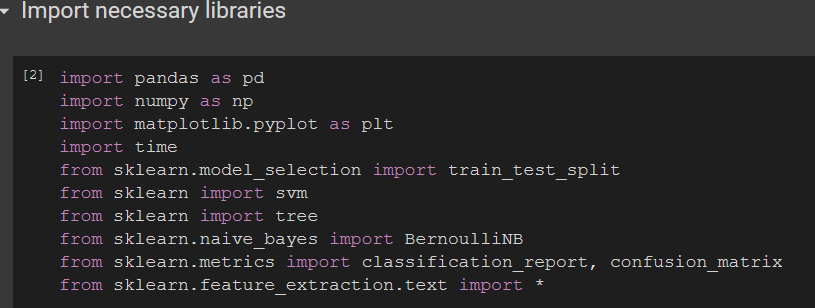
\includegraphics[width=1\textwidth]{import.png}
\vspace{0.3cm}

\noindent
\large{The Python's code above shows all the libraries used for the homework. As shown, \textit{"sklearn"} library is imported to solve the problem, which is a open-source library for machine learning in python, even for beginners. \newline
\textbf{panda:} panda is the famous framework used to work, import, extract data from data-sets; it can be used for every kind of data analysis and manipulation. \newline
Then from sklearn: \newline
\textbf{numpy:} To handle arrays \newline
\textbf{pyplot:} Necessary to print confusion\_matrix \newline
\textbf{time:} Used to measure training computational time of different models. \newline
\textbf{train\_test\_split:} function to split the dataset into random train and test subsets. \newline
\textbf{svm:} Support-vector machines model. \newline
\textbf{tree:} Regression Tree model. \newline
\textbf{naive\_bayes:} Naive Bayes classifier. \newline
\textbf{metrics:} tools to plot classification report and confusion matrix (no plot). \newline
\textbf{feature\_extraction:} library for vectorizers. \newline
\textbf{plot\_confusion\_matrix (not shown)}: Imported function to plot confusion matrix of trained models.
}

\vspace{0.5cm}

\noindent
\textbf{\large{Note:}}\large{ The whole homework has been developed on "Google Colab", firstly to have a smooth "hardware" setup in order to test, run and debug the problem (which could be very slow on a dated computer) and also to add some layout while coding the solution.}

\newpage
\section{Data-set file management}


\vspace{0.4cm}
\hspace{-1.0in}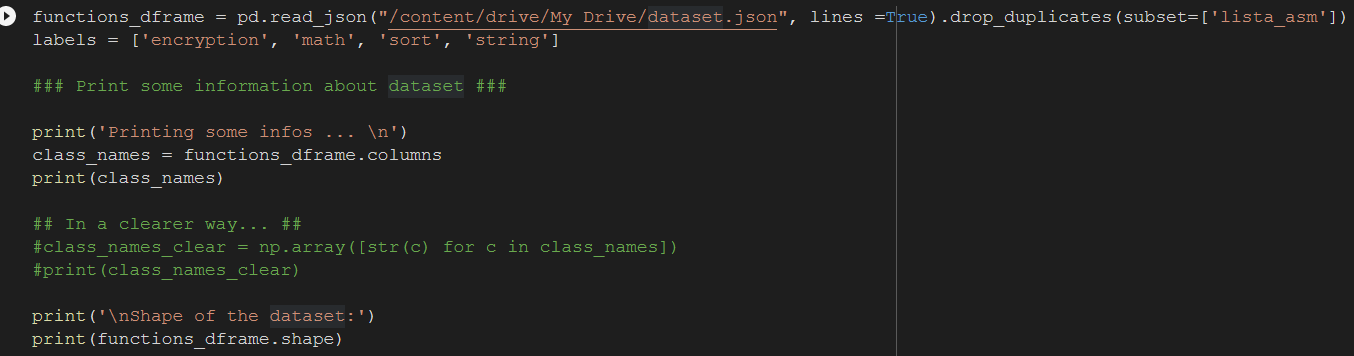
\includegraphics[width=1.3\textwidth]{datasetfile.png}
\vspace{0.3cm}

\noindent
\large{As mentioned, the homework has been developed on Colab: with the first line the script imports the data-set file from the Google Drive folder after prompting a warning for permission; here the file is imported with \textit{read\_json} function with parameter \textit{lines=True}, this implements the import from a JSON Line file. The function saves the data-set on a \textit{pandaframe} from the relative library.\newline
Further on some data-set's info are printed, such features (columns) and shape (Number of lines = data-set's samples, Number of columns = data-set's features). \newline
Other information (not shown in the code above) can be checked removing comments on lines (for example: print the first 5 samples, or samples [300:349]). \newline
}

\vspace{0.5cm}

\noindent
\textbf{\large{Note on drop\_duplicates:}}\large{ \newline
drop\_duplicates function has been added some days later the start of the homework: course's professors communicated that the data-set given is full of duplicates, thus when building and making predictions with the model was possible to have as result really high accuracy (like all '1.00' for test\_set in use); to solve this issue was possible either to try dropping duplicates (and firstly i tried to do so by cycling samples and applying a manual check, but was a heavy  and not optimal solution), or use another data-set given which was free of duplicates \newline
In the end, both data-sets were used to measure performance differences although this was minimal (both data-sets have a shape of 6073 samples).
}

\newpage
\section{Vectorization}

\vspace{0.4cm}
\hspace{+0.2in}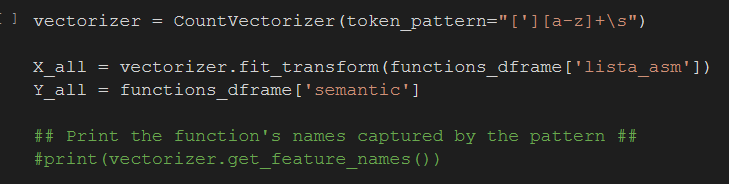
\includegraphics[width=1.0\textwidth]{vectorization.png}
\vspace{0.3cm}

\hspace{-0.2in}\noindent
\large{
In this piece of code the true pre-processing of data takes place. \newline
In the first line \textit{CountVectorizer} is initialized; it provides a simple way to both 'tokenize' a collection of text documents (or, as in this case, a text describing binary functions in assembly) and then build a vocabulary of selected words in order to learn from it how many times a specific \textit{'string'} appears in a specific document and then classify it accordingly. \newline
Then the vectorizer trasforms and fits the values of \textbf{'lista\_asm'} of the dataframe imported from data-set file. At the end the result of this operation along with the values of \textbf{'semantic'} field (labels) are saved in two different variables used later.

\vspace{0.5cm}

\noindent
\textbf{\large{Note on token\_pattern:}}\large{ \newline
Without any setting, CountVectorizer counts every string as a single token for the vocabulary. Before using and setting the token\_pattern value, was tried a manually solution of isolating the necessary words from the lista\_asm camp, indeed this solution was even working but after discovering the possibility of using regex value to 'capture' correct and useful worlds, this solution was removed. \newline
Analyzing the data-set's lista\_asm field, was decided to extract assembly commands called by every sample function (for example: 'call', 'move', 'add', 'pop', 'imul', ...); these commands follows a simple regex's pattern: \newline
Before every command there is a "'" (\textbf{[']} in regex), then a sequence of chars follows (\textbf{[a-z]+} in regex, with the plus meaning at least one) and then a blank space follows as a "string terminator" (\textbf{/s} in regex). \newline
This setting (and intuition) was very helpful to realize a clearer and faster solution.
}

\newpage
\section{Data-set Split}


\vspace{0.4cm}
\hspace{+0.2in}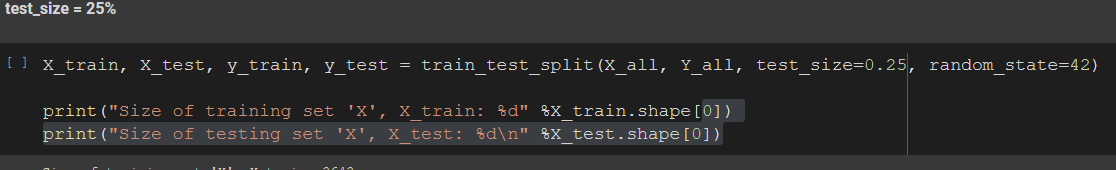
\includegraphics[width=1.0\textwidth]{split.png}
\vspace{0.3cm}

\noindent
\hspace{-0.05in}\large{
In this phase finally the learning part begins: \newline
The pre-processed data is divided into four portions to first train the model and then to evaluate it in order to measure his accuracy and performances:

\begin{itemize}
	\item \textbf{x\_train:} The training set
	\item \textbf{y\_train:} The set of labels to all the data in x\_train
	\item \textbf{x\_test:} Validation set
	\item \textbf{y\_test:} The set of labels to all the data in y\_test
\end{itemize}

\noindent
Also \textbf{X\_all} is the vectorizer after the transformation and \textbf{Y\_all} is the set of labels, both passed as parameter of the split function.
}

\vspace{0.5cm}

\noindent
\textbf{\large{Note:}}\large{ \newline
\textbf{test\_size} and \textbf{random\_state} are also very important parameters: the first describe the percentage of the data-set that will be used as validation set (and of course the rest will be the percentage of training set) while the latter is used as random seed (changing this value will effect which sample will be part of the training set or validation set.)
}
	


\newpage
\section{Decision Trees model}

\begin{center}
\vspace{0.2cm}
\hspace{+0.2in}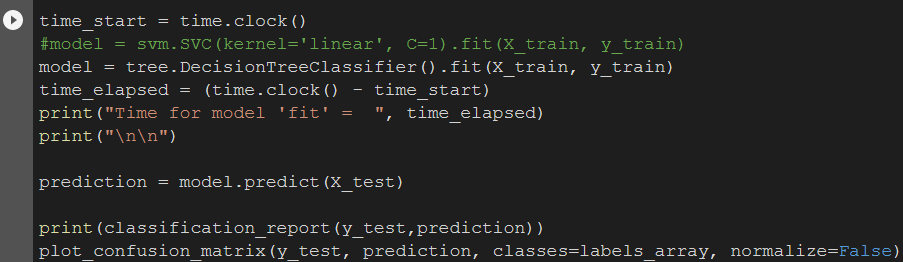
\includegraphics[width=0.7\textwidth]{tree.png}
\vspace{0.1cm}

\vspace{0.1cm}
\hspace{+0.2in}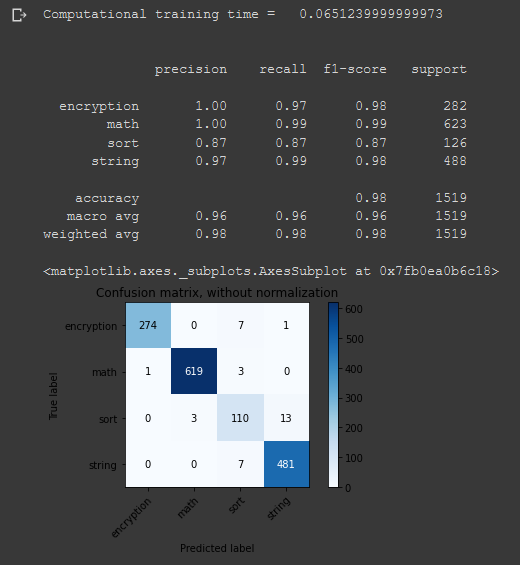
\includegraphics[width=0.7\textwidth]{tree_matrix.png}
\vspace{0.3cm}
\end{center}

\newpage
\section{Bernoulli model}

\begin{center}
	\vspace{0.2cm}
	\hspace{+0.2in}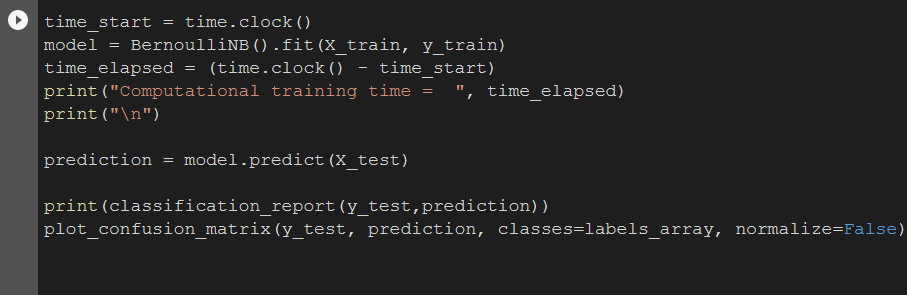
\includegraphics[width=0.7\textwidth]{bernoulli.png}
	\vspace{0.1cm}
	
	\vspace{0.1cm}
	\hspace{+0.2in}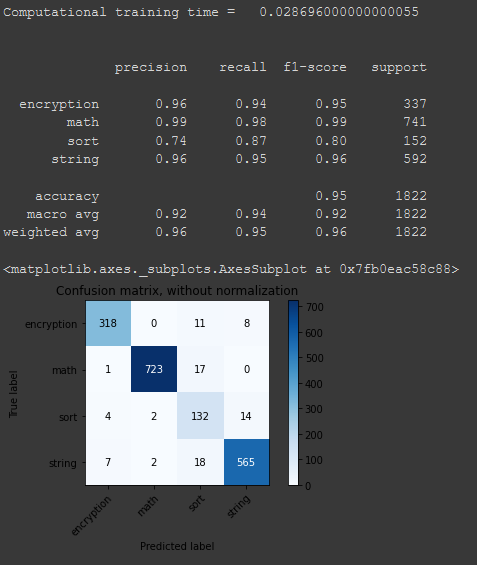
\includegraphics[width=0.7\textwidth]{bernoulli_matrix.png}
	\vspace{0.3cm}
\end{center}

\newpage
\section{Support Vector Machine - Linear}

\begin{center}
	\vspace{0.2cm}
	\hspace{+0.2in}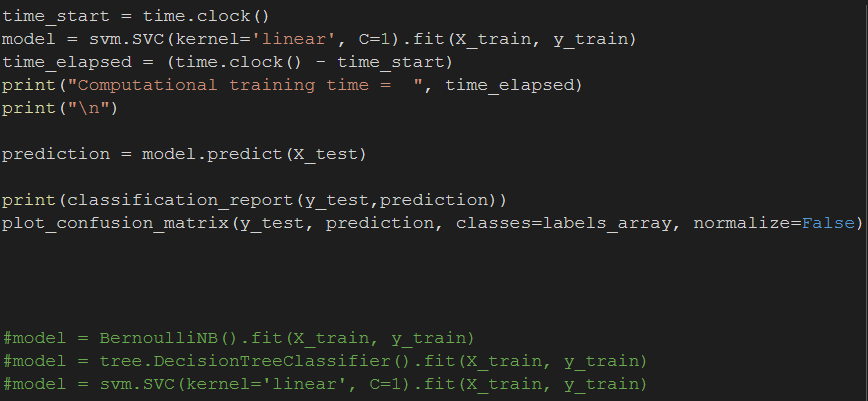
\includegraphics[width=0.7\textwidth]{svm.png}
	\vspace{0.1cm}
	
	\vspace{0.1cm}
	\hspace{+0.2in}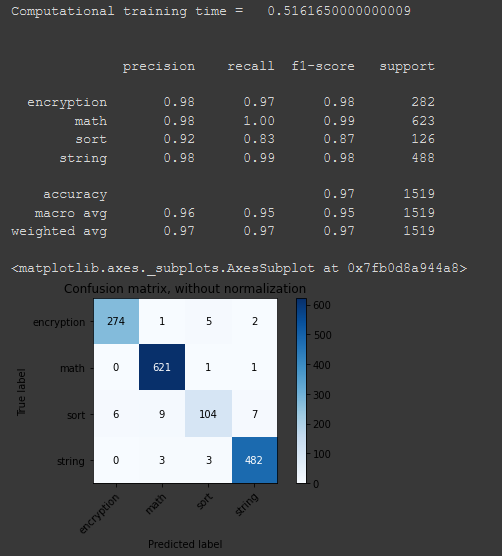
\includegraphics[width=0.7\textwidth]{svm_matrix.png}
	\vspace{0.3cm}
\end{center}

\newpage
\section{Conclusions}
\hspace{-0.05in}\large{

\noindent
\textbf{\large{Note:}} \newline
Every solution adopted for this homework was tested multiple times, both by changing test\_size subset size and random state. Solutions displayed in above pages were computed with a \textbf{test\_size = 0.30} and \textbf{random\_state = 42} (if not mentioned otherwise).

\vspace{0.5cm}

\noindent
As shown in the previous pages, three different approaches were chosen to model this homework and predict the solution.
Firs of all, I tried to model the problem with Decision Trees: honestly i didn't trust much the "good" numbers resulted from the computation; the way the CountVectorizer has been implemented, in my opinion, is not a good way for Decision Trees. This because the solution simply counts the occurrences of every single assembly function called by the sample given; and analyzing the CountVectorizer's items is possible to notice that there are a lot's of functions which are very rare or called just few times: I think that this maybe created a problem of overfitted model, or in another words, the model builds over-complex tree and does not generalize the data well. A solution would be to prune the tree to at least remove features (assembly's function) which have low importance. \newline
This could create other problems thought. As suggested from tips, the data-set has "Math" labeled samples that make huge use of math operations, but suppose that even another function type make use of some math operations mixed with other things: Will the tree simply assign the sample to Math
just because finds a reasonable number of math functions? Maybe cause other features were pruned? \newline
The key is to find balance between a overfitted tree and a not enough "deep" one. Also maybe adding some other elements into the classification process would be useful (for example use of registers and special registers, like "xmm*").
\newline

\noindent
On similar line of Decision Trees, just slightly better, there is Naive Bayes solution, and, to be more precise, BernoulliNB which brings some probability on evaluating the model.\newline
I simply thought that instead of declaring a sample of this or that type basing the prediction only on the occurrences numbers of some functions was not enough to generalize the solution. So i tried to compute the model using only binary occurrence of functions (is this function in the sample?) using BernoulliNB (not multinomial). The data-set is presented with enough level of "separation" ("Math" uses math function, "Sorting" makes huge use of compare and mov*, ...), and so trying this approach seemed a good idea. \newline
In my opinion the solution is still afflicted by some overfitting and as explained before this could be resolved by accounting also registers into CountVectorizers. At the end, though, this approach helped me to realize that "Sort" and "String" samples make use of similar assembly's function, this is an important factor to remind when building a more solid train-set in pre-process phase (some sort/string samples where badly assigned, thus the accuracy decreased slightly).
\newline 

\noindent
Trying to bypass the "overfitted or not" dilemma which is the main protagonist of  this homework, brought me to the idea of implementing Support Vector Machines, thus to have a model with some sort of regularization on parameters. The key here is to choose the right kernel and regularization parameter "C". I trusted the linearity of the data-set given (even on the way it was pre-processed) so i used Linear kernel with "standard" regularization (C=1).
\newline
Results seems very good with this approach, and indeed i felt much more confident that with Decision Trees and Naive Bayes.
}

\vspace{0.5cm}

\noindent
\large{
\hspace{-0.05in}As expected, the computational training time "winner" is the BernoulliNB Model, simply because it accounts much less parameters and tests to evaluate the model. \newline
The loser is of course Decision Tree model, and this slightly confirms the fact that the model is building a "over-complex" tree (overfitted, of course), it's even slower than SVM and his regularization process, I didn't expect it at all!
}

\end{document}